\documentclass{article}

\usepackage{tikz}
\usetikzlibrary{calc}
\begin{document}
\begin{figure}
\tikzset{
tick/.style = {black, very thick}
}

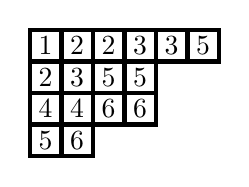
\begin{tikzpicture} % boxlength=0.4%ZEILE NR. 0 (von unten)

%ELEMENT IN SPALTE NR. 0 (von links)
\draw [ultra thick] (0.0,0.0) rectangle (0.4,0.4);
\node at ($(0.2,0.2)$) {$5$};

%ELEMENT IN SPALTE NR. 1 (von links)
\draw [ultra thick] (0.4,0.0) rectangle (0.8,0.4);
\node at ($(0.6000000000000001,0.2)$) {$6$};




%ZEILE NR. 1 (von unten)

%ELEMENT IN SPALTE NR. 0 (von links)
\draw [ultra thick] (0.0,0.4) rectangle (0.4,0.8);
\node at ($(0.2,0.6000000000000001)$) {$4$};

%ELEMENT IN SPALTE NR. 1 (von links)
\draw [ultra thick] (0.4,0.4) rectangle (0.8,0.8);
\node at ($(0.6000000000000001,0.6000000000000001)$) {$4$};

%ELEMENT IN SPALTE NR. 2 (von links)
\draw [ultra thick] (0.8,0.4) rectangle (1.2000000000000002,0.8);
\node at ($(1.0,0.6000000000000001)$) {$6$};

%ELEMENT IN SPALTE NR. 3 (von links)
\draw [ultra thick] (1.2000000000000002,0.4) rectangle (1.6,0.8);
\node at ($(1.4000000000000001,0.6000000000000001)$) {$6$};




%ZEILE NR. 2 (von unten)

%ELEMENT IN SPALTE NR. 0 (von links)
\draw [ultra thick] (0.0,0.8) rectangle (0.4,1.2000000000000002);
\node at ($(0.2,1.0)$) {$2$};

%ELEMENT IN SPALTE NR. 1 (von links)
\draw [ultra thick] (0.4,0.8) rectangle (0.8,1.2000000000000002);
\node at ($(0.6000000000000001,1.0)$) {$3$};

%ELEMENT IN SPALTE NR. 2 (von links)
\draw [ultra thick] (0.8,0.8) rectangle (1.2000000000000002,1.2000000000000002);
\node at ($(1.0,1.0)$) {$5$};

%ELEMENT IN SPALTE NR. 3 (von links)
\draw [ultra thick] (1.2000000000000002,0.8) rectangle (1.6,1.2000000000000002);
\node at ($(1.4000000000000001,1.0)$) {$5$};




%ZEILE NR. 3 (von unten)

%ELEMENT IN SPALTE NR. 0 (von links)
\draw [ultra thick] (0.0,1.2000000000000002) rectangle (0.4,1.6);
\node at ($(0.2,1.4000000000000001)$) {$1$};

%ELEMENT IN SPALTE NR. 1 (von links)
\draw [ultra thick] (0.4,1.2000000000000002) rectangle (0.8,1.6);
\node at ($(0.6000000000000001,1.4000000000000001)$) {$2$};

%ELEMENT IN SPALTE NR. 2 (von links)
\draw [ultra thick] (0.8,1.2000000000000002) rectangle (1.2000000000000002,1.6);
\node at ($(1.0,1.4000000000000001)$) {$2$};

%ELEMENT IN SPALTE NR. 3 (von links)
\draw [ultra thick] (1.2000000000000002,1.2000000000000002) rectangle (1.6,1.6);
\node at ($(1.4000000000000001,1.4000000000000001)$) {$3$};

%ELEMENT IN SPALTE NR. 4 (von links)
\draw [ultra thick] (1.6,1.2000000000000002) rectangle (2.0,1.6);
\node at ($(1.8,1.4000000000000001)$) {$3$};

%ELEMENT IN SPALTE NR. 5 (von links)
\draw [ultra thick] (2.0,1.2000000000000002) rectangle (2.4000000000000004,1.6);
\node at ($(2.2,1.4000000000000001)$) {$5$};







\end{tikzpicture}
\end{figure}
\end{document}

